\documentclass[12pt]{article}
%\usepackage[utf8]{inputenc}
\usepackage{indentfirst}
\usepackage{float}
\usepackage{array}
\usepackage{url}
\urlstyle{tt}
\usepackage{enumitem, amsmath, amssymb, amsfonts, latexsym, mathrsfs}
\usepackage{graphicx}
\usepackage{subfig}
\usepackage{multicol}
\usepackage{booktabs}
\usepackage{ragged2e}
\usepackage{svg}
\usepackage{xcolor}

\usepackage{listings}
\usepackage{atkinson} %% Option 'sfdefault' if the base
%% font of the document is to be sans serif.
\usepackage[T1]{fontenc}
\setmainfont{Atkinson Hyperlegible}
\renewcommand{\familydefault}{\sfdefault}

\usepackage[spanish]{babel}
\usepackage[utf8]{inputenc}
\usepackage[backend=biber]{biblatex}
\bibliography{referencias}
\usepackage{csquotes}
%New colors defined below
\usepackage{}
\definecolor{codegreen}{rgb}{0,0.6,0}
\definecolor{codegray}{rgb}{0.5,0.5,0.5}
\definecolor{codepurple}{rgb}{0.58,0,0.82}
\definecolor{backcolour}{rgb}{0.95,0.95,0.92}
\lstdefinestyle{mystyle}{
  backgroundcolor=\color{backcolour},   commentstyle=\color{codegreen},
  keywordstyle=\color{magenta},
  numberstyle=\tiny\color{codegray},
  stringstyle=\color{codepurple},
  basicstyle=\ttfamily\footnotesize,
  breakatwhitespace=false,         
  breaklines=true,                 
  captionpos=b,                    
  keepspaces=true,                 
  numbers=left,                    
  numbersep=5pt,                  
  showspaces=false,                
  showstringspaces=false,
  showtabs=false,                  
  tabsize=2
}
%"mystyle" code listing set
\lstset{style=mystyle}
%\lstset{basicstyle=\ttfamily\footnotesize,breaklines=true}

\usepackage{notoccite}

\usepackage{multicol}
\setlength{\columnseprule}{1pt}
\def\columnseprulecolor{\color{black}}





\date{}
% Comand para keywords
\providecommand{\keywords}[1]
{
  \small	
  \textbf{\textit{Keywords---}} #1
}

% Tipografía
%\usepackage{helvet}
%\renewcommand{\familydefault}{\sfdefault}
%\usepackage[sfdefault]{Chivo}
%\usepackage{comment}


\urlstyle{same}
% \tolerance=9999
% \emergencystretch=10pt
\hyphenpenalty=10000
\sloppy
% \exhyphenpenalty=100

\renewcommand{\figurename}{\textbf{Figura.}}
\renewcommand\spanishtablename{Tabla.}

% Interlineado
\usepackage{setspace}
\spacing{1.15}

% Márgenes
\usepackage[a4paper]{geometry}
\geometry{top=2.5cm, bottom=2.5cm, left=2cm, right=2cm}

% Número de página
\usepackage{fancyhdr}
\pagestyle{fancy}
\rhead[]{}
\lhead[]{}
\renewcommand{\headrulewidth}{0pt}
\rfoot[]{\thepage}
\cfoot[]{}

\usepackage[breaklinks]{hyperref}
% Setup de hiperenlaces
\hypersetup{
    colorlinks=true,
    linkcolor=blue,
    filecolor=magenta,      
    urlcolor=cyan,
    pdftitle={Arquitectura de las consolas de videojuegos},
    pdfpagemode=FullScreen,
    citecolor = green
    }
\usepackage[norule]{footmisc}

%_____________________________________________________________________________
%_____________________________________________________________________________
%_____________________________________________________________________________
%_____________________________________________________________________________
\hbadness=50000
\usepackage{microtype}
\begin{document}
\nocite{atkinson}
% PORTADA        
\begin{titlepage}
        \begin{center}
             
         
        \hrule
        \vspace{1cm}
        %{\bfseries\Large UNIVERSIDAT JAUME I \par}
        \vspace{1cm}
        {\bfseries\huge Apuntes de Consolas y Dispositivos de Videojuegos \par}
        \vspace{2cm}

        \begin{figure}[H]
            \centering
            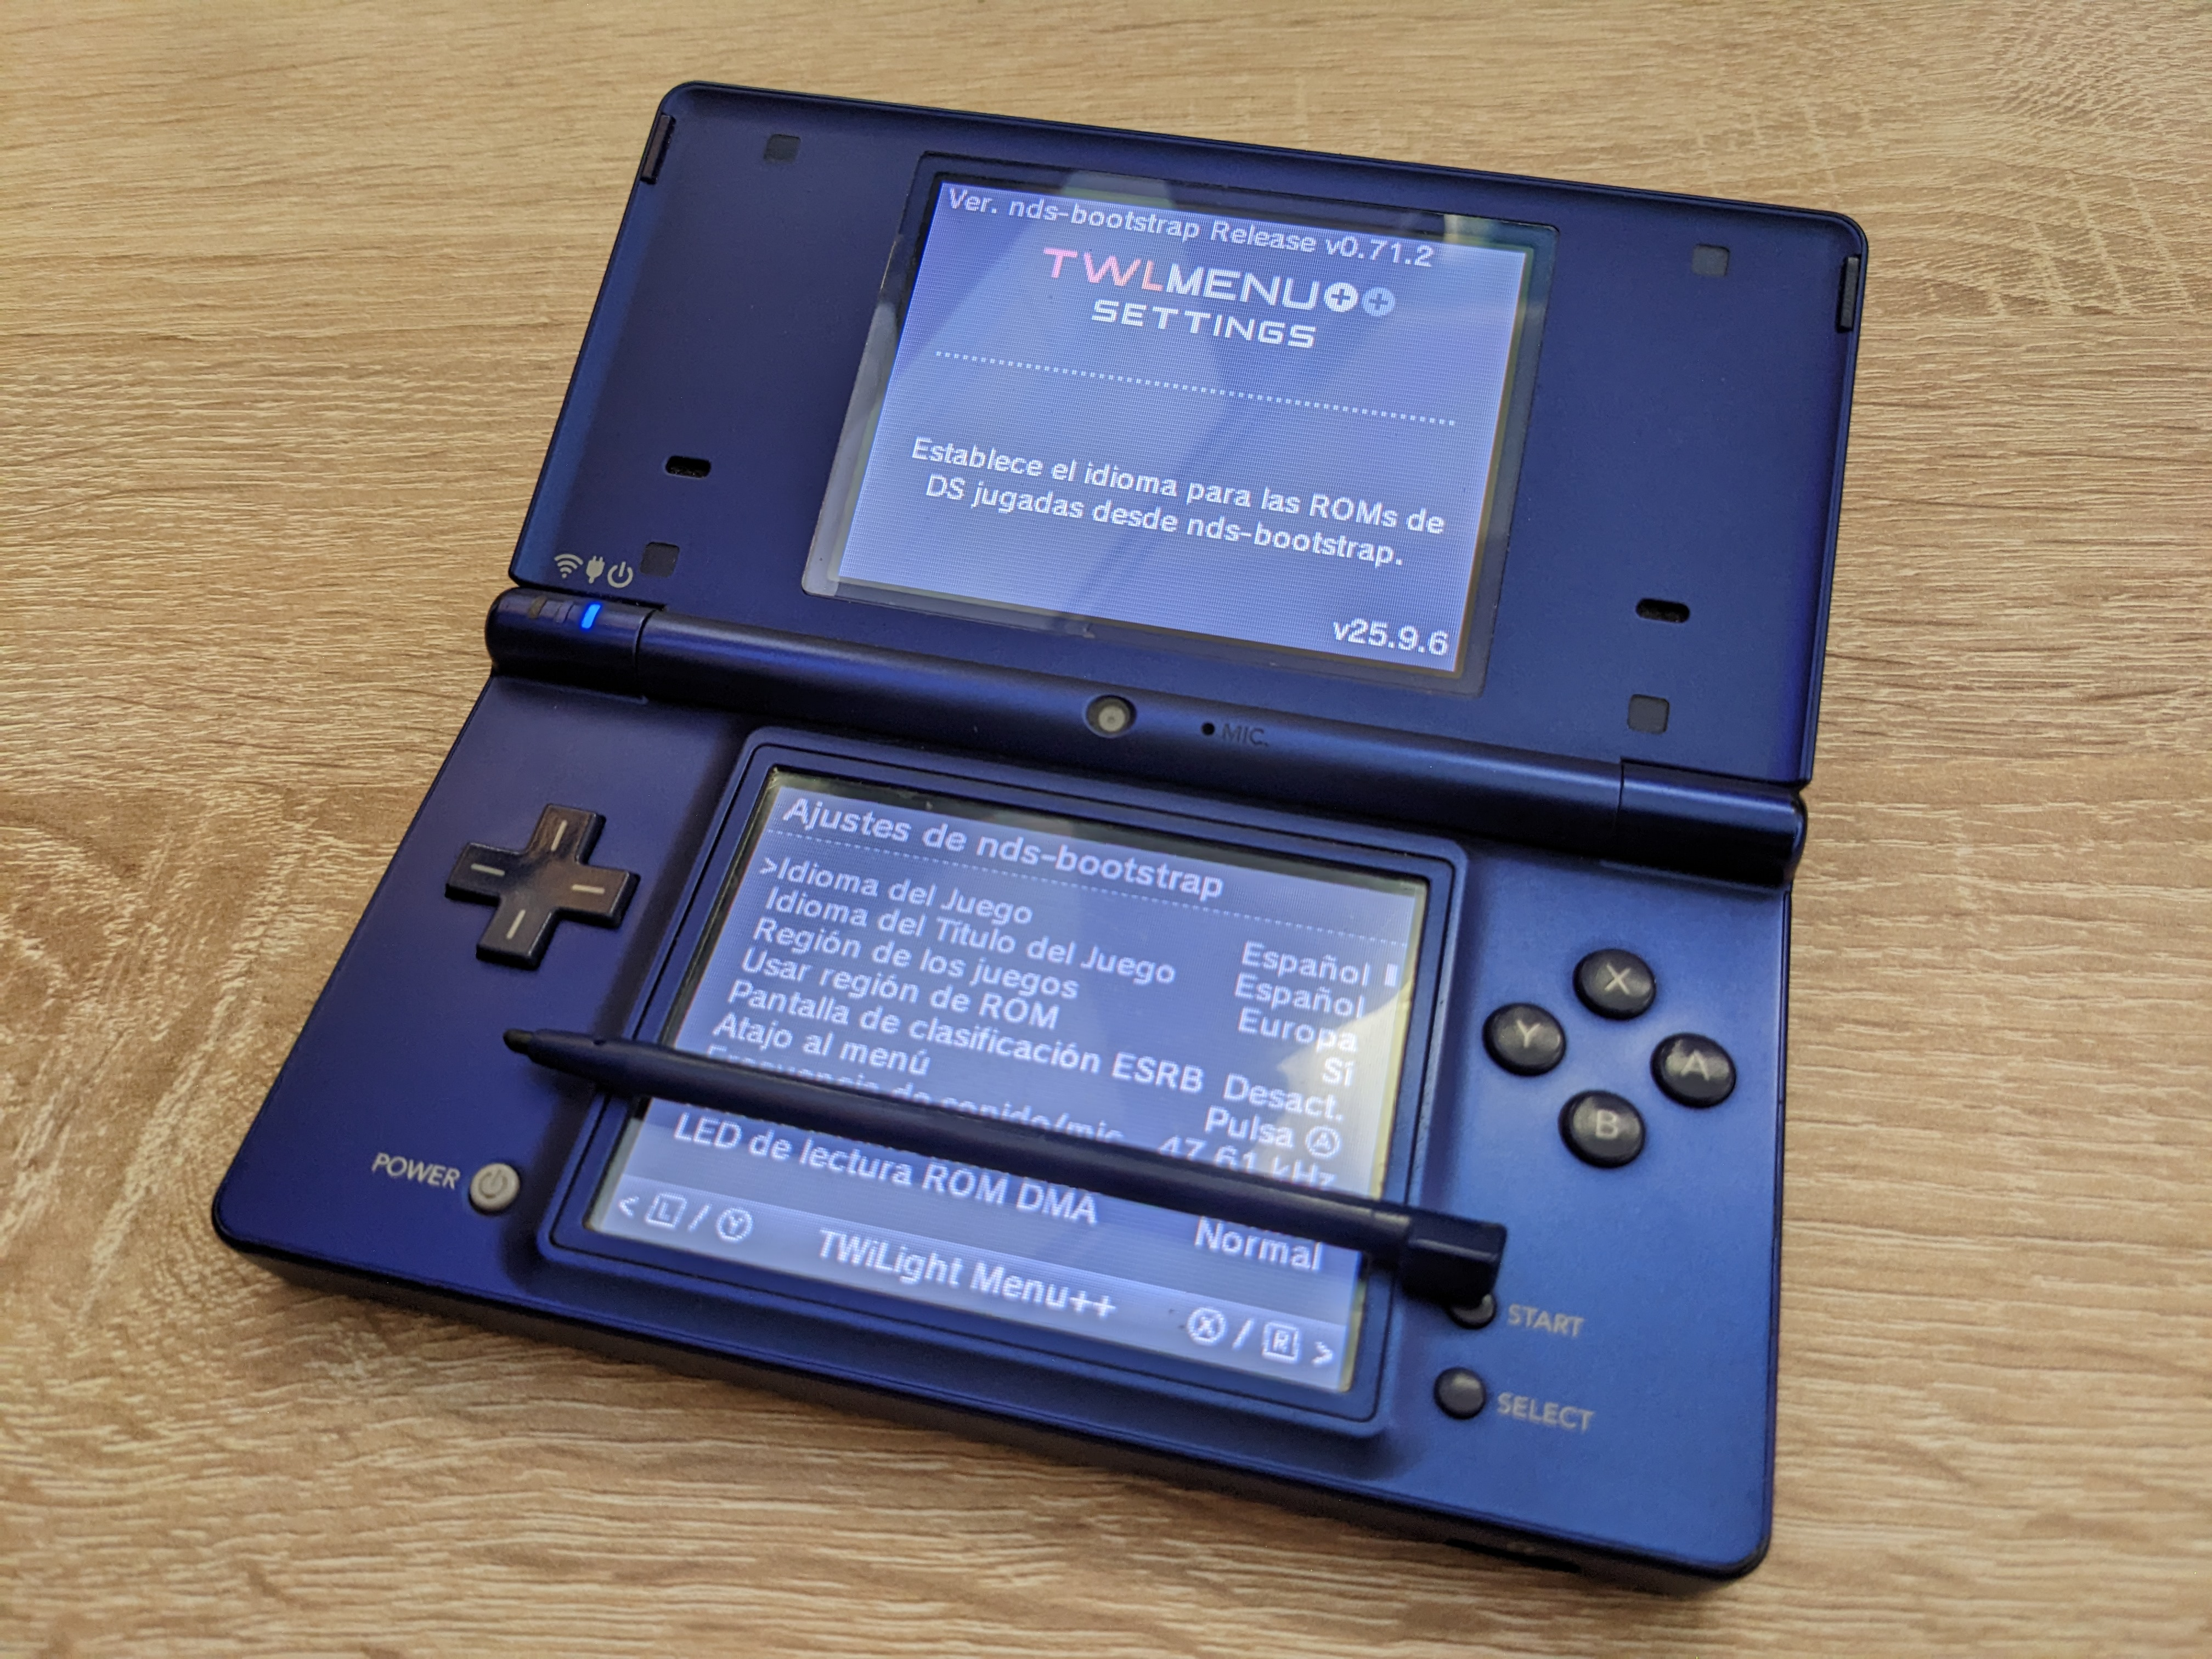
\includegraphics[width=\textwidth]{PXL_20230917_103129958.NIGHT.jpg}
            \caption*{\footnotesize{\textit{Nintendo DSi con Homebrew y emulador de NDS}}}
            \label{fig:dsi}
        \end{figure}
        
        {\large 
        Jesús Jiménez Montero \\
        \par}
        \vspace{1cm}
        \hrule
        \vspace{1cm}

        {\large 
        \textit{Versión 2: Puertas lógicas básicas\\
        Fecha: 24/09/2023}
        \par}
        \end{center}
\end{titlepage}

% ÍNDICE
%\renewcommand{\tableofcontents}{Indice general}
\newpage
\renewcommand{\contentsname}{Tabla de contenidos}
\setcounter{secnumdepth}{5}
\tableofcontents
\setcounter{tocdepth}{4}

\newpage
%-----------------------------------------------------------------
%-----------------------------------------------------------------
% Tabla de figuras
\newpage
\renewcommand{\listfigurename}{Lista de figuras}
\thispagestyle{empty}
\listoffigures
\newpage

\renewcommand{\listtablename}{Lista de tablas}
\listoftables
\newpage

%-----------------------------------------------------------------
%-----------------------------------------------------------------

\section{Puertas lógicas básicas \cite{floyd_fundamentos_2006}} 
    \subsection{NOT}
        \subsubsection{Descripción y tabla de verdad}
            El circuito NOT (o inversor) cambia un nivel lógico al nivel opuesto. En términos de bits, cambia el 1 or el 0 y el 0 por 1. 
            Básicamente, invierte el resultado de la entrada, si A es 1, el inversor lo convierte en 0. 
            % Please add the following required packages to your document preamble:
            % \usepackage{graphicx}
            \begin{table}[H]
            \centering
            \caption{Tabla de verdad de NOT}
            \label{tab:not}
            \resizebox{0.10\linewidth}{!}{%
            \begin{tabular}{l|l}
            A & $\overline{A}$\\ \hline
            0 & 1            \\
            1 & 0           
            \end{tabular}%
            }
            \end{table}
        \subsubsection{Esquema exterior del circuito}
            \begin{figure}[H]
                \centering
                \includesvg{not_exit.svg}
                \caption{Diagrama externo del circuito NOT} \cite{diagram}
                \label{fig:enter-label}
            \end{figure}
        \subsubsection{Esquema interior del circuito}
            \begin{figure}[H]
                \centering
                \includesvg{NOT.svg}
                \caption{Diagrama interno del circuito NOT} \cite{diagram}
                \label{fig:enter-label}
            \end{figure}
        \newpage \subsubsection{Código HDL}
            \begin{lstlisting}
    /**
     * Not gate:
     * out = not in
     */
    
    CHIP Not {
        IN in;
        OUT out;
    
        PARTS:
            Nand(a=in,b=in,out=out);
    }
            \end{lstlisting}
    \newpage
    \subsection{AND}
        \subsubsection{Descripción y tabla de verdad}
            La puerta AND es la puerta básica de todas con la que se contruyen el resto de puertas lógicas. Puede tener dos o más entradas y realiza la multiplicación lógica.
            La puerta AND de dos entradas, produce 1 la salida si A y B son 1. La salida será 0 si A es 0, o si B es 0, o ambas son 0. 
            % Please add the following required packages to your document preamble:
            % \usepackage{graphicx}
            \begin{table}[H]
            \centering
            \caption{Tabla de verdad de AND}
            \label{tab:AND}
            \resizebox{0.25\linewidth}{!}{%
            \begin{tabular}{ll|l}
            \multicolumn{2}{l|}{Entrada} & Salida \\
            A             & B            & X      \\ \hline
            0             & 0            & 0      \\
            0             & 1            & 0      \\
            1             & 0            & 1      \\
            1             & 1            & 1     
            \end{tabular}%
            }
            \end{table}
        \subsubsection{Esquema exterior del circuito}
            \begin{figure}[H]
                \centering
                \includesvg{and_extern.svg}
                \caption{Diagrama externo del circuito AND} \cite{diagram}
                \label{fig:enter-label}
            \end{figure}
        
        \subsubsection{Esquema interior del circuito}
            \begin{figure}[H]
                \centering
                \includesvg{and_inter.svg}
                \caption{Diagrama interno del circuito AND} \cite{diagram}
                \label{fig:enter-label} 
            \end{figure}
        \newpage \subsubsection{Código HDL}
            \begin{lstlisting}
     /**
     * And gate:
     * out = 1 if (a == 1 and b == 1) / 0 otherwise
     */
    
    CHIP And {
      IN a, b;
      OUT out;
    
      PARTS:
          Nand(a=a, b=b, out=n);
          Nand(a=n, b=n, out=out);
    } 
            \end{lstlisting}
    \newpage  
    
    \subsection{OR}
        \subsubsection{Descripción y tabla de verdad}
            La puerta OR es otra de las puertas básicas para construir funciones lógicas. También tienen 2 o más entradas y hace la operación lógica de suma.
            En una puerta OR, la salida es 1 si cualquiera de las entradas A o B, o ambas, son 1. La salida será 0 si ambas entradas, A y B, están a 0. 

            % Please add the following required packages to your document preamble:
            % \usepackage{graphicx}
            \begin{table}[H]
            \centering
            \caption{Tabla de verdad de OR}
            \label{tab:OR}
            \resizebox{0.25\linewidth}{!}{%
            \begin{tabular}{ll|l}
            \multicolumn{2}{l|}{Entrada} & Salida \\
            A             & B            & X      \\ \hline
            0             & 0            & 0      \\
            0             & 1            & 1      \\
            1             & 0            & 1      \\
            1             & 1            & 1     
            \end{tabular}%
            }
            \end{table}
        \subsubsection{Esquema exterior del circuito}
            \begin{figure}[H]
                \centering
                \includesvg{or_exter.svg}
                \caption{Diagrama externo del circuito OR} \cite{diagram}
                \label{fig:enter-label}
            \end{figure}
        \subsubsection{Esquema interior del circuito}
            \begin{figure}[H]
                \centering
                \includesvg{or_inter.svg}
                \caption{Diagrama interno del circuito OR} \cite{diagram}
                \label{fig:enter-label}
            \end{figure}
        \newpage \subsubsection{Código HDL}  
        \begin{lstlisting}
     /**
     * Or gate:
     * out = 1 if (a == 1 or b == 1)
     *       0 otherwise
     */
    
    CHIP Or {
        IN a, b;
        OUT out; 
        
        PARTS:
            Nand(a=a,b=a,out=c);
            Nand(a=b,b=b,out=d);
            Nand(a=c,b=d,out=out);
    }
        \end{lstlisting}
    \newpage
    \subsection{XOR}

        \subsubsection{Descripción y tabla de verdad}
            En un XOR (OR-Exclusiva), la salida es 1 si A es 0 y la B es 1; además también la salida será 1 si A es 1 y B a 1. La salida será 0 si tanto A y B son también 0.
            
            El resultado es 0 si todos los términos son iguales y 1 si cualquier término es diferente.
            $F(A,B) = XOR(A,B)$

            % Please add the following required packages to your document preamble:
            % \usepackage{graphicx}
            \begin{table}[H]
            \centering
            \caption{Tabla de verdad de XOR}
            \label{tab:XOR}
            \resizebox{0.25\linewidth}{!}{%
            \begin{tabular}{ll|l}
            \multicolumn{2}{l|}{Entrada} & Salida \\
            A             & B            & X      \\ \hline
            0             & 0            & 0      \\
            0             & 1            & 1      \\
            1             & 0            & 1      \\
            1             & 1            & 0     
            \end{tabular}%
            }
            \end{table}
        \subsubsection{Esquema exterior del circuito}
            \begin{figure}[H]
                \centering
                \includesvg{xor_exter.svg}
                \caption{Diagrama externo del circuito XOR} \cite{diagram}
                \label{fig:enter-label}
            \end{figure}
        \subsubsection{Esquema interior del circuito}
            \begin{figure}[H]
                \centering
                \includesvg{xor_inter.svg}
                \caption{Diagrama interno del circuito XOR} \cite{diagram}
                \label{fig:enter-label}
            \end{figure}
        \newpage \subsubsection{Código HDL}  
        \begin{lstlisting}
    /**
     * Exclusive-or gate:
     * out = not (a == b)
     */
    
    CHIP Xor {
            IN a, b;
            OUT out;
        
        PARTS:
            Not(in=a,out=na);
            Not(in=b,out=nb);
            And(a=na,b=b,out=c);
            And(a=a,b=nb,out=d);
            Or(a=c,b=d,out=out);
}
        \end{lstlisting}
    \newpage
    \subsection{MUX / Multiplexor}
        \subsubsection{Descripción y tabla de verdad}

            El multiplexor (MUX) permite dirigir información procedente de diversas fuentes a una sola línea para llegar a un destino común. Al MUX también pueden conmutar las entradas de datos hacia la salida. Además, se les conoce como selectores de datos. 
            % Please add the following required packages to your document preamble:
            % \usepackage{graphicx}
            \begin{table}[H]
            \centering
            \caption{Tabla de verdad de MUX}
            \label{tab:mux}
            \resizebox{0.25\linewidth}{!}{%
            \begin{tabular}{l|lll}
            A & B & sel & out \\ \hline
            0 & 0 & 0   & 0   \\
            0 & 1 & 0   & 0   \\
            1 & 0 & 0   & 1   \\
            1 & 1 & 0   & 1   \\
            0 & 0 & 1   & 0   \\
            0 & 1 & 1   & 1   \\
            1 & 0 & 1   & 0   \\
            1 & 1 & 1   & 1  
            \end{tabular}%
            }
            \end{table}
        \subsubsection{Esquema exterior del circuito}
            \begin{figure}[H]
                \centering
                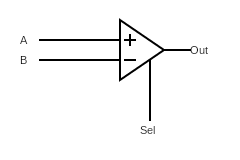
\includegraphics{mux_ext.png}
                \caption{Diagrama externo del circuito MUX} \cite{diagram}
                \label{fig:mux_ext}
            \end{figure}
        \subsubsection{Esquema interior del circuito}
            \begin{figure}[H]
                \centering
                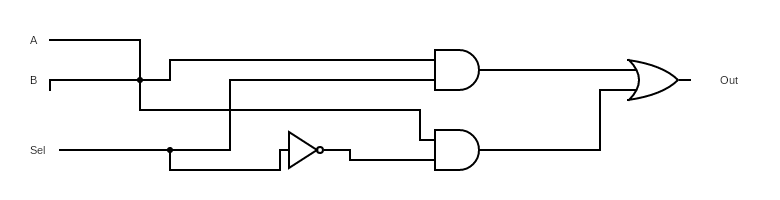
\includegraphics[width=0.5\linewidth]{mux_int.png}
                \caption{Diagrama interior de circuito MUX} \cite{diagram}
                \label{fig:mux_int}
            \end{figure}
        \subsubsection{Código HDL}  

            \begin{lstlisting}
     /** 
     * Multiplexor:
     * out = a if sel == 0
     *       b otherwise
     */
    
    CHIP Mux {
        IN a, b, sel;
        OUT out;
    
        PARTS:
            Not(in=sel,out=nsel);
            And(a=a,b=nsel,out=c);
            And(a=b,b=sel,out=d);
            Or(a=c,b=d,out=out);
    }
            \end{lstlisting}

    \newpage
    \subsection{DMUX / Demultiplexor}
        \subsubsection{Descripción y tabla de verdad}
            El demultiplexor (DMUX / DEMUX \cite{floyd_fundamentos_2006}), hace la función contraria del multiplexor; toma datos de una línea y los distribuye a un número determinado de salidas. También se le conoce como distribuidor de datos. 

            % Please add the following required packages to your document preamble:
            % \usepackage{graphicx}
            \begin{table}[H]
            \centering
            \caption{Tabla de verdad de DMUX}
            \label{tab:dmux}
            \resizebox{0.25\linewidth}{!}{%
            \begin{tabular}{ll|ll}
            in & sel & A & B \\ \hline
            0  & 0   & 0 & 0 \\
            0  & 1   & 0 & 0 \\
            1  & 0   & 1 & 0 \\
            1  & 1   & 0 & 1
            \end{tabular}%
            }
            \end{table}
        \subsubsection{Esquema exterior del circuito}
            \begin{figure}[H]
                \centering
                \includesvg{dmux_ext.svg}
                \caption{Diagrama externo del circuito DMUX} \cite{diagram}
                \label{fig:dmux_ext}
            \end{figure}
        \subsubsection{Esquema interior del circuito}
            \begin{figure}[H]
                \centering
                \includesvg{dmux_int.svg}
                \caption{Diagrama interno del circuito DMUX} \cite{diagram}
                \label{fig:enter-label}
            \end{figure}
        \newpage \subsubsection{Código HDL}  
        \begin{lstlisting}
/**
 * Demultiplexor:
 * {a, b} = {in, 0} if sel == 0
 *          {0, in} if sel == 1
 */

CHIP DMux {
    IN in, sel;
    OUT a, b;

    PARTS:
        Not(in=sel,out=nsel);
        And(a=in,b=nsel,out=a);
        And(a=in,b=sel,out=b);
}
        \end{lstlisting}
    \newpage

\printbibliography[heading=bibintoc]
\end{document}
